\chapter{Materiales, Métodos e Implementación}

\section{Materiales}
\label{section4:materials}
Para la realización de este TFM se dispone de una colección de 497 modelos 3D de la sínfisis del pubis, correspondientes tanto al lado izquierdo como derecho, en formato de malla OBJ. Estos modelos fueron escaneados por el personal del Laboratorio de Antropología Física del Departamento de Medicina Legal, Toxicología y Antropología Física de la Universidad de Granada. Además de la digitalización tridimensional, el equipo del laboratorio examinó cuidadosamente cada una de las muestras y etiquetó manualmente los atributos correspondientes a las características morfológicas observables en la superficie de la sínfisis del pubis así como la edad real de fallecimiento de los individuos, datos que también han sido provistos dentro de un fichero de Microsoft Excel.

\begin{figure}[h]
    \centering
    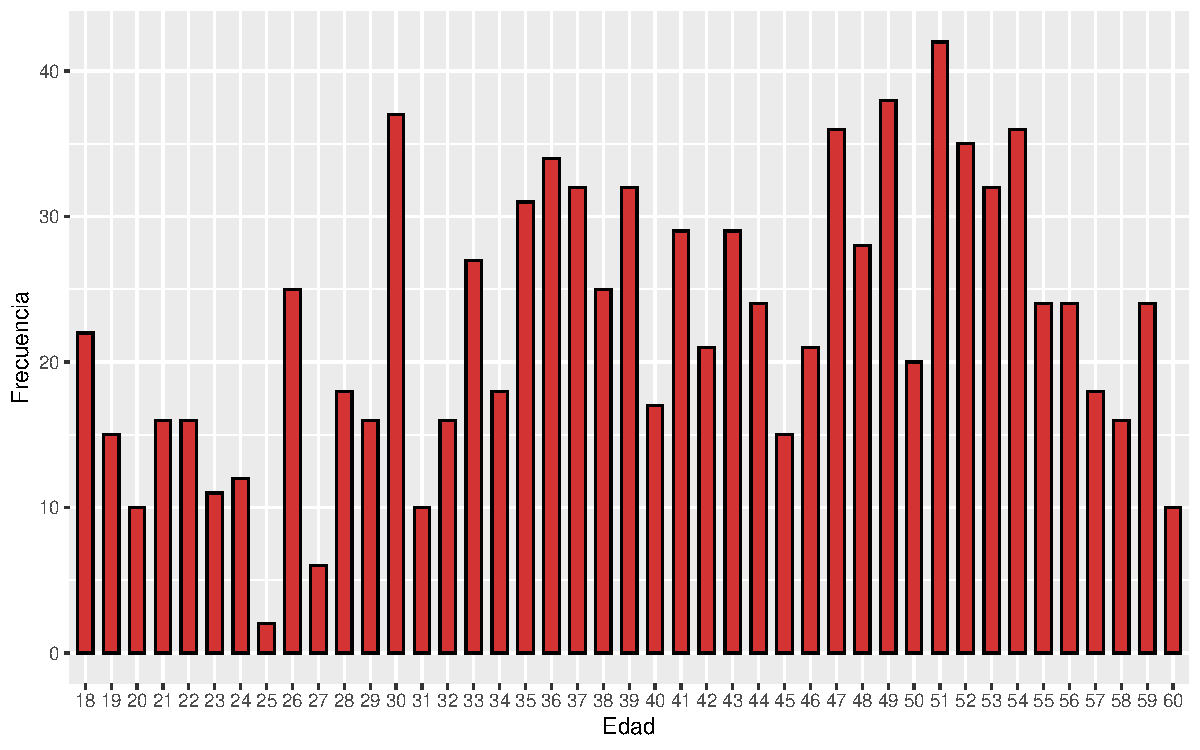
\includegraphics[width=\linewidth]{../../scripts/eda/eda_univar/char_age_distr.pdf}
    \caption[Distribución de los datos por edad]{Distribución de los datos las edades conocidas de los sujetos}
    \label{fig4:age}
\end{figure}
\begin{figure}[h]
    \centering
    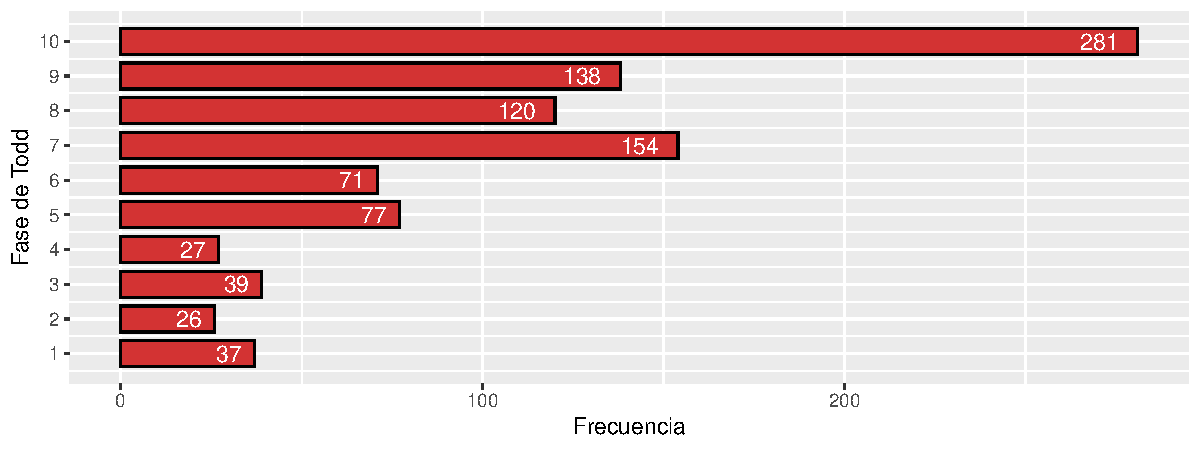
\includegraphics[width=\linewidth]{../../scripts/eda/eda_univar/char_t_phase_distr.pdf}
    \caption[Distribución de los datos por cada rango de edad]{Distribución de los datos por cada rango de edad del método de Todd. \textbf{1}: 18-19 años, \textbf{2}: 20-21 años, \textbf{3}: 22-24 años, \textbf{4}: 25-26 años, \textbf{5}: 27-30 años, \textbf{6}: 30-35 años, \textbf{7}: 35-39 años, \textbf{8}: 39-44 años, \textbf{9}: 45-50 años, \textbf{10}: 50+ años.}
    \label{fig4:todd_phase}
\end{figure}

\subsection{Análisis Exploratorio de Datos}
Realizando un análisis exploratorio de los datos (\textit{Exploratory Data Analisys}, EDA), se observa que la muestra está compuesta por individuos de entre 18 y 60 años, como se muestra en la Figura \ref{fig4:age}. Además, estos individuos han sido clasificados dentro de las 10 fases del método de Todd, tal como se aprecia en la Figura \ref{fig4:todd_phase}.

De ambos gráficos se aprecia que las edades más representadas corresponden a individuos de mayor edad, lo cual es coherente considerando el origen de los datos. Sin embargo, este patrón también evidencia un desbalance inherente en la muestra, un fenómeno esperado cuando se trabaja con datos reales.

\subsubsection{Análisis Univariable}
Continuando con el EDA enfocado en las nueve características del método de Todd, se observa un claro desbalance en la distribución de clases, como se muestra en las gráficas correspondientes en la Figura \ref{fig4:todd_chars}. Las clases más representadas son coherentes con las manifestaciones morfológicas que el hueso de la sínfisis del pubis presenta a edades más avanzadas.

Desde la perspectiva del balance de datos, las características de Borde Dorsal (Subfigura \ref{fig4:todd_chars__use}), Nódulo Óseo (Subfigura \ref{fig4:todd_chars__bn}), Plataforma Dorsal (Subfigura \ref{fig4:todd_chars__dp}) y Borde Inferior (Subfigura \ref{fig4:todd_chars__lse}) presentan un desbalance particularmente acentuado, con aproximadamente 95\%, 91\%, 90\% y 90\% de las muestras concentradas en una sola clase, respectivamente. Este fuerte desbalance sugiere que estas características podrían tener un rendimiento limitado al ser utilizadas para el entrenamiento de modelos de DL.

\begin{figure}[p]
    \centering
    \begin{subfigure}{\textwidth}
        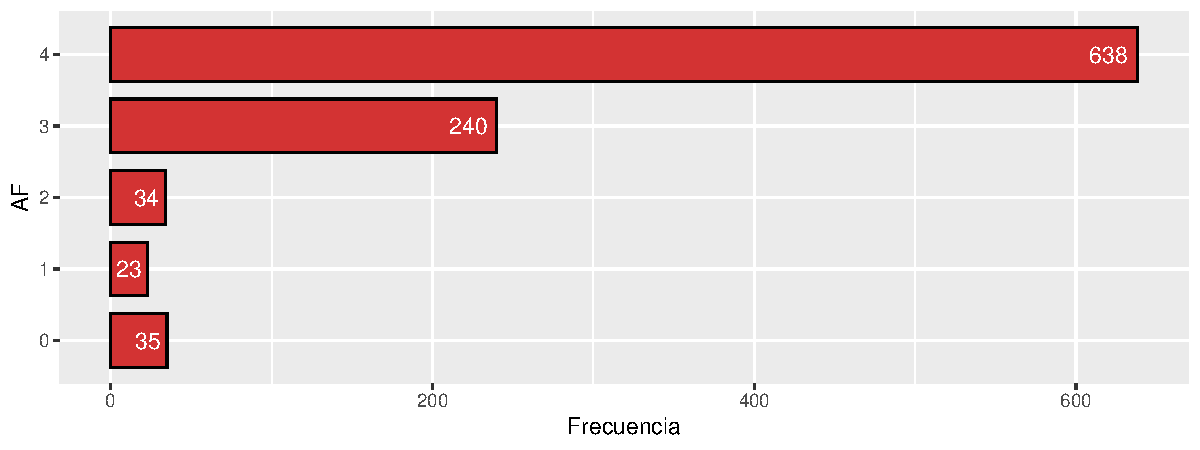
\includegraphics[width=\linewidth]{../../scripts/eda/eda_univar/char_af_distr.pdf}
        \caption{Crestas y Surcos (\textit{Auricular Face}, AF)}
        \label{fig4:todd_chars__af}
    \end{subfigure}

    \begin{subfigure}{\textwidth}
        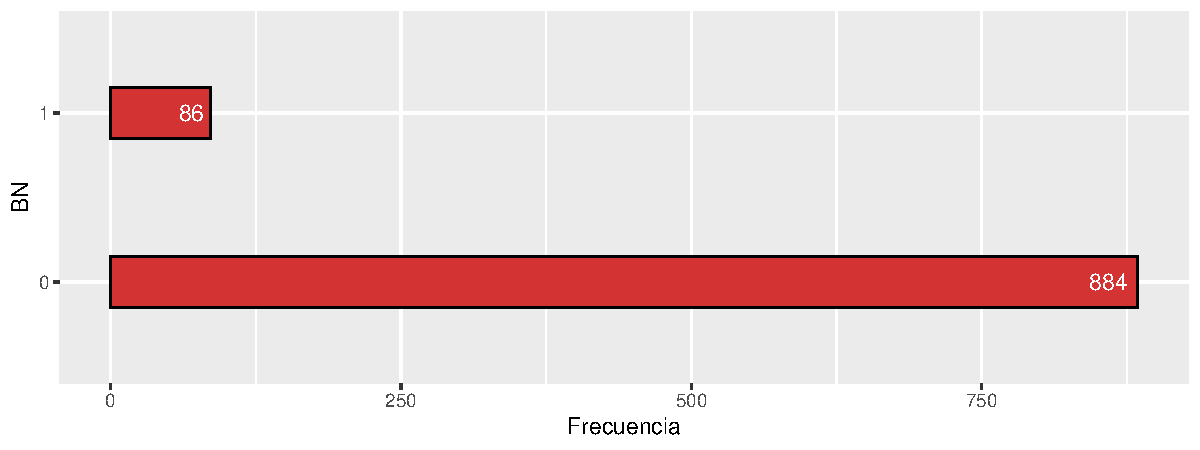
\includegraphics[width=\linewidth]{../../scripts/eda/eda_univar/char_bn_distr.pdf}
        \caption{Nódulo Óseo (\textit{Bony Nodule}, BN)}
        \label{fig4:todd_chars__bn}
    \end{subfigure}
    
    \begin{subfigure}{\textwidth}
        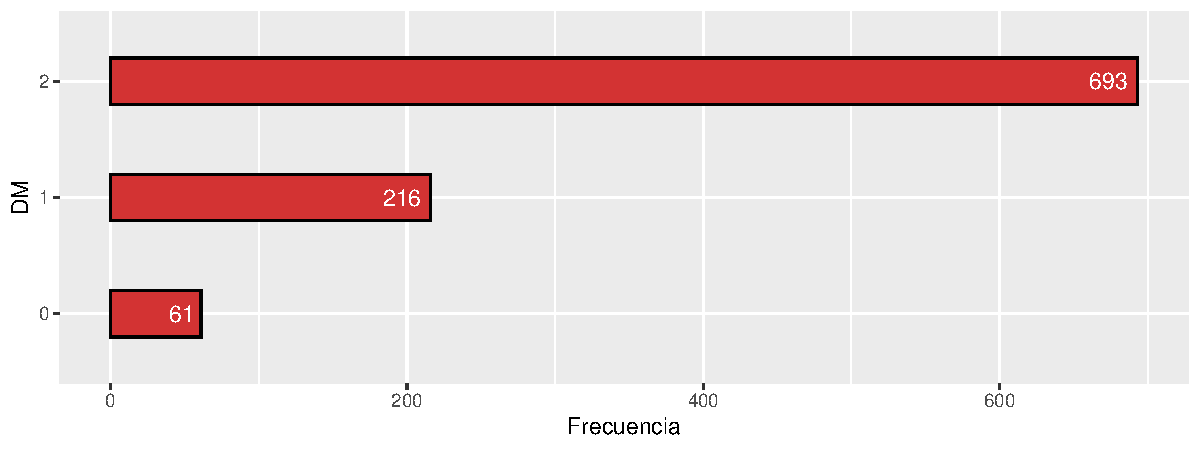
\includegraphics[width=\linewidth]{../../scripts/eda/eda_univar/char_dm_distr.pdf}
        \caption{Borde Dorsal (\textit{Dorsal Margin}, DM)}
        \label{fig4:todd_chars__dm}
    \end{subfigure}
    \phantomcaption

\end{figure}
\begin{figure}[p]
    \ContinuedFloat

    \begin{subfigure}{\textwidth}
        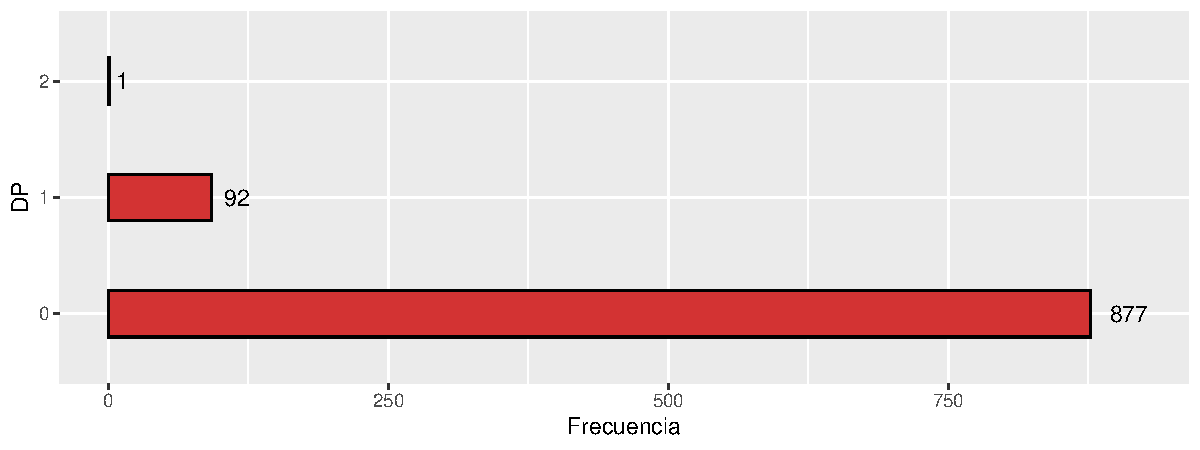
\includegraphics[width=\linewidth]{../../scripts/eda/eda_univar/char_dp_distr.pdf}
        \caption{Plataforma Dorsal (\textit{Dorsal Plateau}, DP)}
        \label{fig4:todd_chars__dp}
    \end{subfigure}

    \begin{subfigure}{\textwidth}
        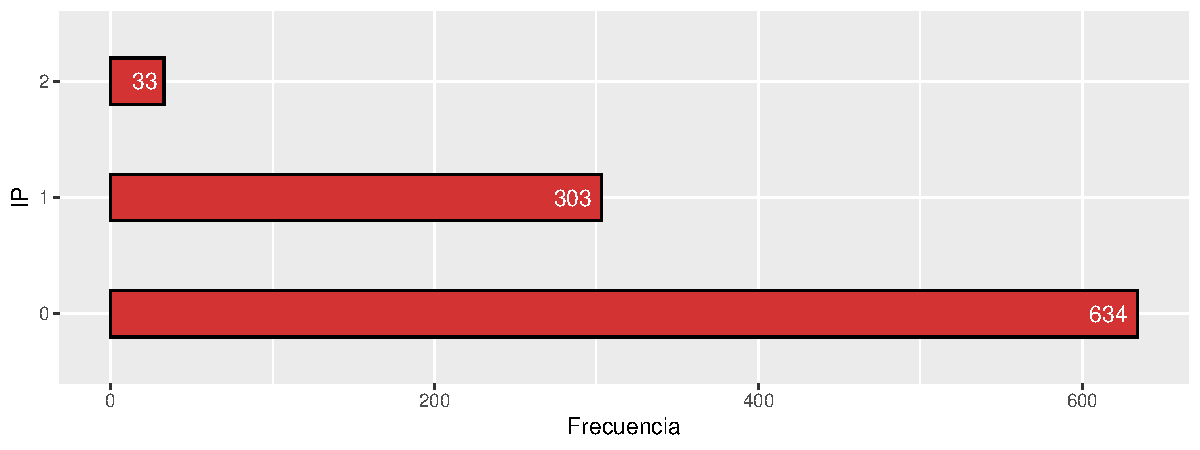
\includegraphics[width=\linewidth]{../../scripts/eda/eda_univar/char_ip_distr.pdf}
        \caption{Porosidad Irregular (\textit{Irregular Porosity}, IP)}
        \label{fig4:todd_chars__ip}
    \end{subfigure}

    \begin{subfigure}{\textwidth}
        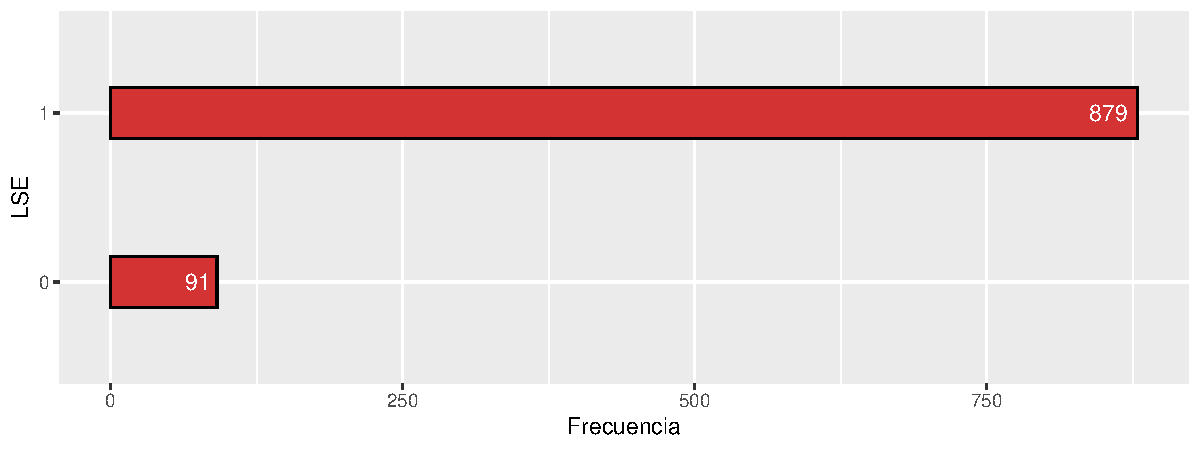
\includegraphics[width=\linewidth]{../../scripts/eda/eda_univar/char_lse_distr.pdf}
        \caption{Borde Inferior (\textit{Lower Symphysial Extremity}, LSE)}
        \label{fig4:todd_chars__lse}
    \end{subfigure}

    \phantomcaption
    \label{fig4:todd_chars}
\end{figure}
\begin{figure}[p]
    \ContinuedFloat

    \begin{subfigure}{\textwidth}
        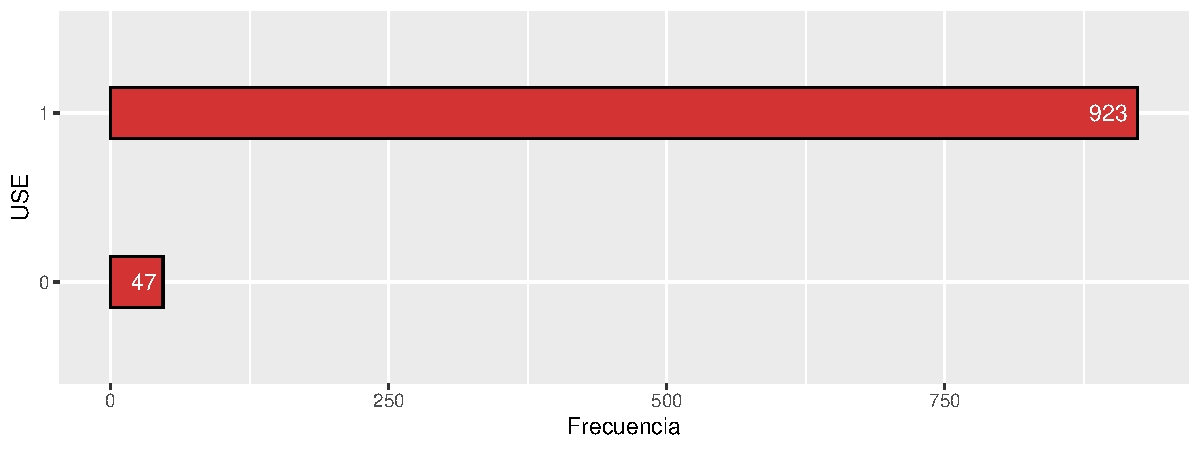
\includegraphics[width=\linewidth]{../../scripts/eda/eda_univar/char_use_distr.pdf}
        \caption{Borde Dorsal (\textit{Upper Symphysial Extremity}, USE)}
        \label{fig4:todd_chars__use}
    \end{subfigure}

    \begin{subfigure}{\textwidth}
        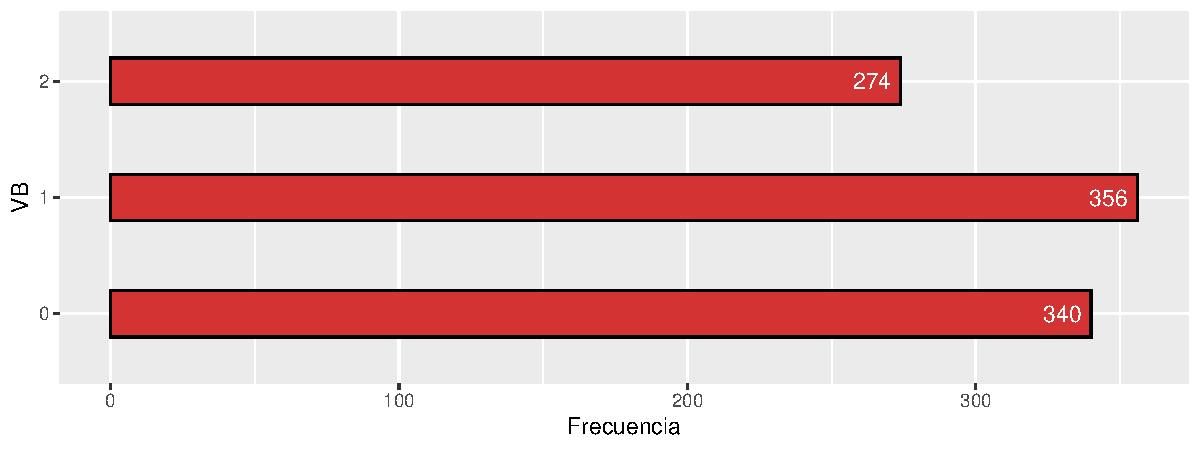
\includegraphics[width=\linewidth]{../../scripts/eda/eda_univar/char_vb_distr.pdf}
        \caption{Bisel Ventral (\textit{Ventral Bevel}, VB)}
        \label{fig4:todd_chars__vb}
    \end{subfigure}

    \begin{subfigure}{\textwidth}
        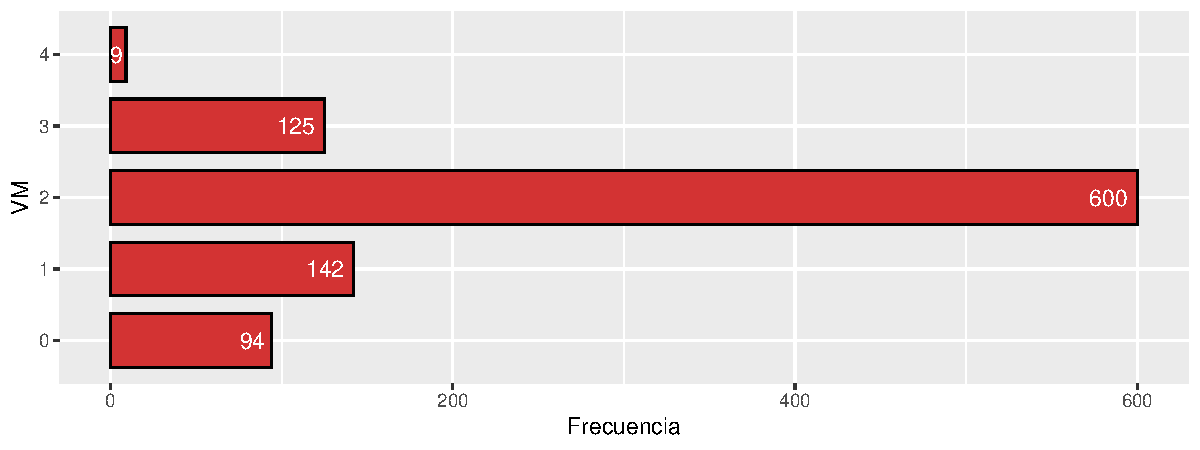
\includegraphics[width=\linewidth]{../../scripts/eda/eda_univar/char_vm_distr.pdf}
        \caption{Borde Ventral (\textit{Ventral Margin}, VM)}
        \label{fig4:todd_chars__vm}
    \end{subfigure}
    \caption[Distribución de las características de Todd]{Distribución de las características de Todd en los datos}

\end{figure}

El resto de las características muestra un desbalance menos extremo, con entre el 60\% y el 70\% de los datos agrupados en una única clase. La característica con mayor equilibrio en su distribución es el Bisel Ventral (Subfigura \ref{fig4:todd_chars__vb}), en la que los datos se reparten aproximadamente en un 33\% por clase, dado que esta posee tres clases distintas. Se espera que esta característica, junto con aquellas que presenten menos desbalance, proveerán mejores resultados al ser entrenadas por la red.

\subsubsection{Correlaciones}

\begin{figure}[p]
    \centering
    \begin{subfigure}{\textwidth}
        \centering
        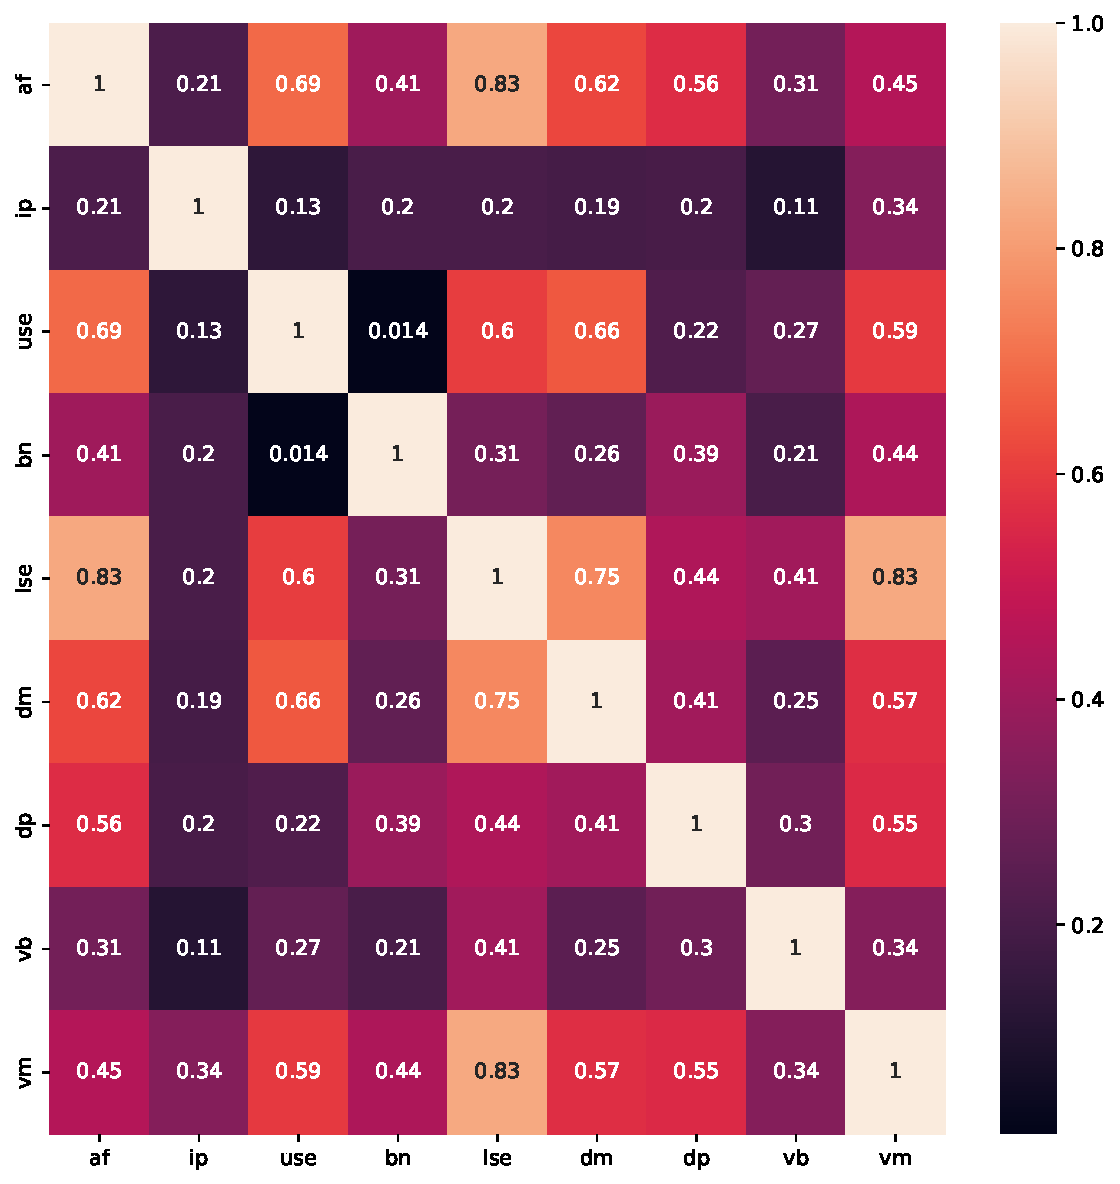
\includegraphics[width=0.7\linewidth]{../../scripts/eda/assoc_plot_cramersv.pdf}
        \caption{Correlograma usando la V de Cramér}
        \label{fig4:todd_chars__cramersv}
    \end{subfigure}
    \begin{subfigure}{\textwidth}
        \centering
        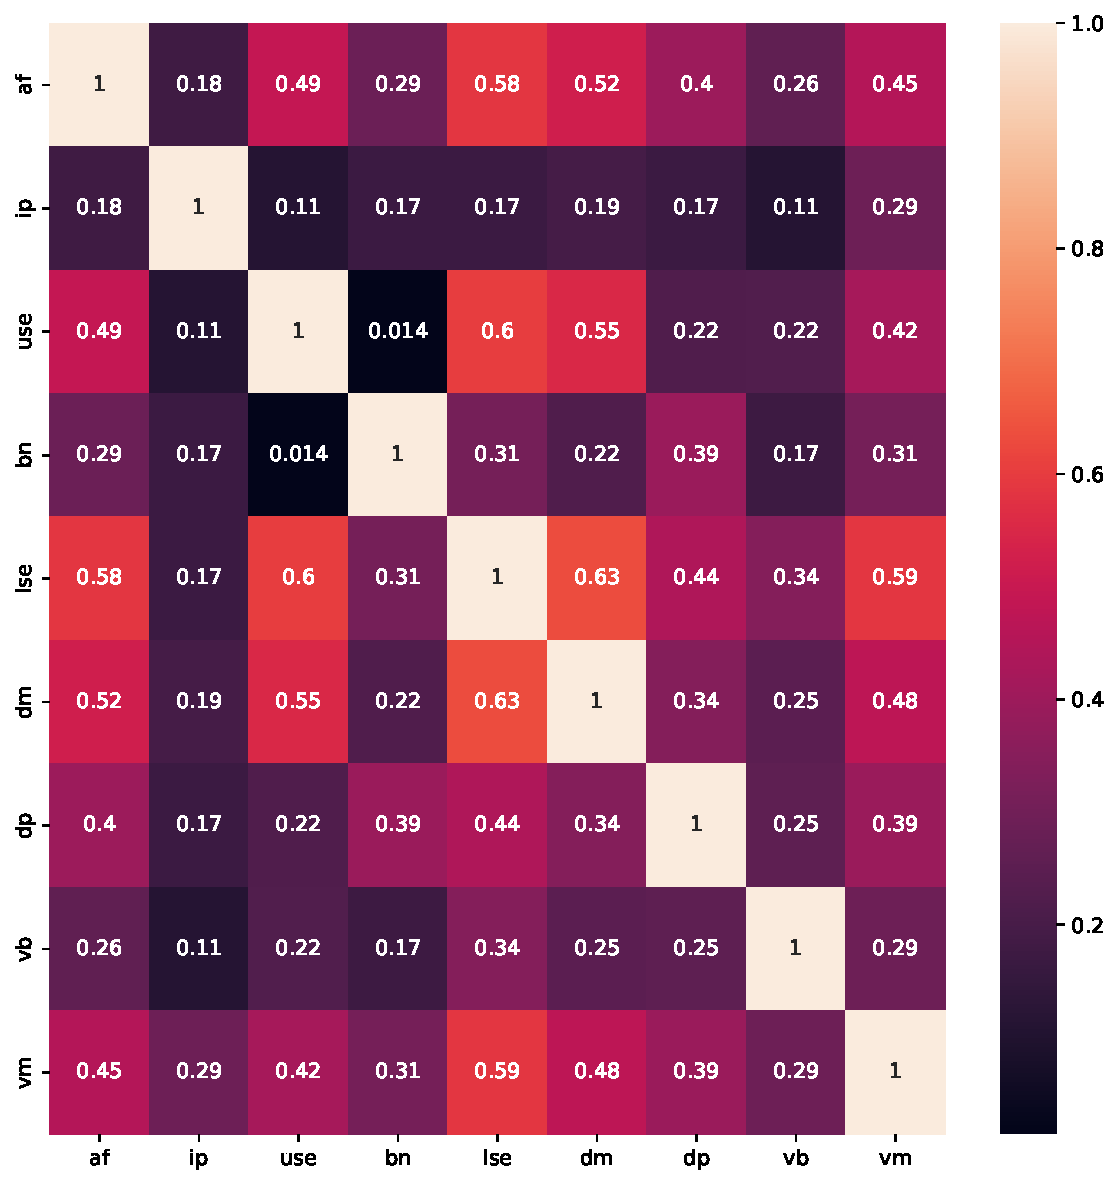
\includegraphics[width=0.7\linewidth]{../../scripts/eda/assoc_plot_tschuprow.pdf}
        \caption{Correlograma usando la T de Tschuprow}
        \label{fig4:todd_chars__tschuprow}
    \end{subfigure}
    \caption[Correlogramas entre características de Todd]{Correlogramas entre las características de Todd}
    \label{fig4:todd_chars_correlogram}
\end{figure}

Si bien los datos empleados en este estudio no son de naturaleza tabular y se utilizan técnicas de DL que no requieren una extracción manual de características, resulta igualmente útil de cara a los experimentos analizar las correlaciones existentes entre las nueve características de Todd. Dado que dichas variables son categóricas, se ha optado por utilizar la V de Cramér, una medida estadística que cuantifica el grado de asociación entre dos variables categóricas. Además, para corregir el sesgo que puede surgir al trabajar con tablas de contingencia no cuadradas, se ha complementado el análisis con la T de Tschuprow, la cual atenúa dicho efecto y permite una interpretación más equilibrada de la asociación entre las variables.

Ambos correlogramas se presentan en la Figura \ref{fig4:todd_chars_correlogram}, donde puede apreciarse que las correlaciones entre las características de Todd varían significativamente entre sí. Como era de esperarse, existen discrepancias entre los valores obtenidos mediante la V de Cramér y la T de Tschuprow, siendo esta última más conservadora en presencia de tablas de contingencia no cuadradas. Para facilitar la interpretación de estos resultados, se ha incluido la Tabla \ref{table4:corr}, en la que se listan las tres características con mayor correlación para cada una.

Del análisis se concluye que las características LSE, AF y VM son, en general, las que presentan los mayores niveles de correlación con el resto, lo que sugiere una mayor dependencia entre ellas. En contraste, la característica IP muestra los niveles más bajos de correlación con las demás, seguida de BN, lo cual puede indicar un comportamiento más independiente. Este conocimiento será especialmente relevante en los experimentos de entrenamiento en modo multietiqueta, ya que incorporar características correlacionadas entre sí podría favorecer el aprendizaje del modelo y mejorar su rendimiento.

\begin{table}[t]
    \centering
    \begin{tabular}{|c|cc|}
    \hline
    \rowcolor[HTML]{D33333} 
    \cellcolor[HTML]{D33333}{\color[HTML]{FFFFFF} } & \multicolumn{2}{c|}{\cellcolor[HTML]{D33333}{\color[HTML]{FFFFFF} Características con mayor asociación}} \\ \cline{2-3} 
    \rowcolor[HTML]{D33333} 
    \multirow{-2}{*}{\cellcolor[HTML]{D33333}{\color[HTML]{FFFFFF} Característica}} & \multicolumn{1}{c|}{\cellcolor[HTML]{D33333}{\color[HTML]{FFFFFF} V de Cramér}} & {\color[HTML]{FFFFFF} T de Tschuprow} \\ \hline
    AF & \multicolumn{1}{c|}{LSE, USE, DM} & LSE, DM, USE \\
    BN & \multicolumn{1}{c|}{\textbf{VM, AF, DP}} & \textbf{DP, LSE, VM} \\
    DM & \multicolumn{1}{c|}{LSE, USE, AF} & LSE, USE, AF \\
    DP & \multicolumn{1}{c|}{\textbf{AF, VM, LSE}} & \textbf{LSE, AF, BN} \\
    IP & \multicolumn{1}{c|}{\textbf{VM, AF, LSE}} & \textbf{VM, DM, AF} \\
    LSE & \multicolumn{1}{c|}{\textbf{VM, AF, DM}} & \textbf{DM, USE, VM} \\
    USE & \multicolumn{1}{c|}{AF, DM, LSE} & LSE, DM, AF \\
    VB & \multicolumn{1}{c|}{LSE, VM, AF} & LSE, VM, AF \\
    VM & \multicolumn{1}{c|}{\textbf{LSE, USE, DM}} & \textbf{LSE, DM, AF} \\ \hline
    \end{tabular}
    \caption[Cuadro resumen de las correlaciones más fuertes entre características de Todd]{Cuadro resumen de las correlaciones más fuertes entre cada característica de Todd. Las filas en negrita indican que las características más correladas son diferentes dependiendo del método.}
    \label{table4:corr}
\end{table}

\subsubsection{Preparación de los datos}
\label{section4:data_preparation}
De la muestra original de 497 individuos, es decir, un total de 986 huesos correspondientes a las sínfisis del pubis izquierda y derecha, fue necesario eliminar 16 muestras por diversos motivos: presencia de deformidades anatómicas, ausencia del archivo OBJ asociado o falta de correspondencia entre el modelo 3D y los datos etiquetados provistos. Se opta por utilizar las 970 muestras restantes en su totalidad, ya que en problemas de DL es fundamental contar con un volumen de datos considerable, aunque estos estén altamente desbalanceados, pues se pueden utilizar diversas técnicas para mitigar el efecto que produce esto al rendimiento de un modelo. 

Cabe destacar que, en el caso de la característica Plataforma Dorsal (Subfigura \ref{fig4:todd_chars__dp}), la clase 3 (\say{Presente}) cuenta con solo una muestra, lo cual impide que el modelo pueda aprender representaciones significativas para dicha clase. Por tanto, esta muestra será eliminada durante el entrenamiento de modelos de DL que hagan uso de dicha característica. Además, la Clase 2 originalmente denominada \say{En Formación} será renombrada a \say{Presente}, con el objetivo de mantener la consistencia semántica.

Las 970 mallas presentan una resolución media de 994,601 triángulos, con un mínimo de 329,438 y un máximo de 1,688,348 triángulos. Para poder aplicar el método ExMeshCNN, descrito en la Sección \ref{section4:methods}, es necesario que todas las mallas tengan una resolución uniforme. Una opción inicial considerada fue remuestrear las mallas al número medio de triángulos; sin embargo, este tamaño resulta inviable computacionalmente con el hardware disponible.

Por esta razón, se ha procedido a reducir la resolución de las mallas a 100,000, 50,000 y 25,000 triángulos, empleando las técnicas detalladas en la Sección \ref{section4:data_reduction}. Tal como se demuestra en los experimentos descritos en la Sección \ref{section5:experiment_edge_collapse}, esta reducción no compromete significativamente la fidelidad de la superficie original. La variación entre las superficies del modelo original y las versiones reducidas es mínima, lo que permite afirmar que las mallas simplificadas conservan en mayor o menor grado parte de la información morfológica relevante para los experimentos.

Adicionalmente, el método requiere que las mallas no contengan geometría degenerada y que estén completamente selladas (es decir, que no exista geometría \textit{non-manifold} y que sea \textit{watertight}, según la terminología en gráficos por ordenador). Dado que estas mallas provienen de escaneos de objetos anatómicos reales, es esperable que algunas presenten incompletitud o defectos estructurales, lo que impide su uso directo con ExMeshCNN. Para solventar estos problemas, se aplicaron técnicas de reparación y sellado descritas en la Sección \ref{section4:data_repair}, con el objetivo de restaurar la geometría y garantizar la integridad topológica de cada modelo antes de ser procesado por la red neuronal.

\section{Métodos}
\label{section4:methods}
Como se ha mencionado previamente en la Sección \ref{section3:meshes}, ExMeshCNN \cite{kim_exmeshcnn_2022} representa el estado del arte en el procesamiento de mallas poligonales mediante DL y por lo tanto ha sido el método elegido para realizar los experimentos. A continuación se describe de qué forma el \textit{framework} adapta los datos para poder ser utilizados con convoluciones.

\subsection{Capa de descriptores}
Las representaciones en cuadrícula, como en el caso de imágenes, resultan convenientes porque encapsulan tanto la información de conectividad (es decir, la vecindad local entre píxeles) como las características asociadas (como los valores RGB) en una única estructura matricial. Sin embargo, esta estrategia no puede trasladarse directamente a las mallas tridimensionales debido a su naturaleza irregular y a la ausencia de un orden canónico entre sus elementos.

Para abordar esta limitación, se introducen dos capas iniciales en la red, denominadas descriptores, las cuales contienen parámetros entrenables. El propósito de estas capas es extraer características directamente desde la malla, independientemente del orden de sus triángulos. Estos descriptores transforman la información de la malla a un formato compatible con operaciones de convolución 1D, permitiendo que el modelo aprenda efectivamente a partir de la estructura tridimensional sin requerir una representación regular.

\subsubsection{Descriptor geodésico basado en aristas}
El objetivo de este descriptor es capturar características geodésicas locales asociadas a los triángulos de la malla, características que han sido mayoritariamente ignoradas en la literatura actual. 

Se parte del concepto de distancia geodésica entre caras, definida como el camino más corto a través de aristas que conecta el centro de un triángulo objetivo con un vértice de un triángulo adyacente, pasando por uno de los vértices del triángulo objetivo. No obstante, en mallas triangulares esta métrica resulta limitada, ya que la cantidad de aristas involucradas en dichos caminos es siempre dos, lo cual no aporta mucha información.

Para enriquecer esta representación, se incorporan ideas provenientes de la convolución geodésica propuesta por Schult et al. \cite{schult_dualconvmesh-net_2020}, que toma en cuenta no solo la longitud del camino, sino también su curvatura. De este modo, dos caminos con la misma longitud, pero distinta curvatura permiten ser diferenciados.

Sin embargo, dicha convolución geodésica presenta una limitación importante: la ambigüedad en el orden de los caminos posibles. Dado que estos no poseen una estructura de vecindad ordenada, una misma operación de convolución puede producir diferentes resultados dependiendo del orden de los elementos procesados, comprometiendo así la consistencia del aprendizaje.

Partiendo de estas ideas, se propone el siguiente descriptor $\mathcal{K}$, definido en la Ecuación \ref{eq4:geodesic}:
\begin{equation}
\label{eq4:geodesic}
    \mathcal{K}
(\bar{\textbf{a}_{t}}) = \theta_{0} \sum_{j}^{3} \textbf{u}_{t}^{j} + \theta_{1} \sum_{j}^{3}  \overrightarrow{\textbf{n}}_{t}^{j} + \theta_{2} \sum_{j}^{3} |\textbf{e}_{n(t)}^{j,1} - \textbf{e}_{n(t)}^{j,2}|
\end{equation}
Donde: 
\begin{itemize}
    \item $\bar{\textbf{a}_{t}}$ representa el conjunto conformado por un triángulo objetivo $f_{t}$ y sus tres triángulos vecinos topológicos $f_{n(t)_j}$, con $j \in \left\{1,2,3\right\}$.
    \item $\textbf{u}_{t}^{j}$ describe la relación entre el centro del triángulo $\textbf{c}_t$ y el vértice $j$-ésimo $\textbf{v}_{t}^j$ definido como  $\textbf{u}_{t}^{j} = \textbf{c}_t - \textbf{v}_t^j$ con $j \in \left\{1,2,3\right\}$.
    \item $\overrightarrow{\textbf{n}}_{t}^{j}$ es la normal del vértice $\textbf{v}_t^j$, calculada como la media de las normales de los triángulos que rodean dicho vértice.
    \item $\textbf{e}_{n(t)}^{j,k}$ representa la arista entre el vértice $\textbf{v}_{t}^j$ del triángulo objetivo y un vértice $\textbf{v}_{n(t)}^{j,k}$ del triángulo vecino, donde $k \in \left\{1,2\right\}$. Dado que solo existen dos caminos posibles desde un vértice $\textbf{v}_t^j$ hacia vértices de triángulos vecinos a través de una arista común, la diferencia $|\textbf{e}_{n(t)}^{j,1} - \textbf{e}_{n(t)}^{j,2}|$ captura una característica invariante al orden debido al valor absoluto.
    \item Los términos $\theta_0, \theta_1 $ y $\theta_2$ son parámetros entrenables por la red.
\end{itemize}
Para una mejor comprensión de estos términos, se recomienda consultar la Figura ???.

En esencia, lo que se realiza es un mapeo del triángulo objetivo y su vecindario topológico a un espacio de características geodésicas capturando las siguientes propiedades:
\begin{itemize}
    \item Forma local del triángulo, mediante el término $\textbf{u}_{t}^{j}$, que describe cómo se distribuyen espacialmente los vértices con respecto al centroide.
    \item Orientación local, reflejada en $\overrightarrow{\textbf{n}}_{t}^{j}$, que aporta información sobre la dirección normal de la superficie.
    \item Relaciones geodésicas entre triángulos vecinos, a través del término $|\textbf{e}_{n(t)}^{j,1} - \textbf{e}_{n(t)}^{j,2}|$, que captura la variación entre las conexiones posible
\end{itemize}

Además, el descriptor actúa funcionalmente como un filtro de convolución 1D de tamaño 3, ya que posee parámetros entrenables. Esto permite realizar subsiguientes convoluciones 1D sobre el vector de características obtenido.

\subsubsection{Descriptor geométrico basado en caras}
En la literatura, las características geométricas más comúnmente empleadas para describir las caras triangulares incluyen el vector normal de la misma, su centroide y el ángulo que forma con las caras vecinas. Dado que estas características son de bajo nivel y, en cierta medida, de naturaleza heurística, se propone el descriptor $\mathcal{G}$, definido en la Ecuación \ref{eq4:geometric}, con el objetivo de capturar representaciones de alto nivel que integren dicha información geométrica.

\begin{equation}
\label{eq4:geometric}
    \mathcal{G}(\bar{\textbf{a}_{t}}) = \phi_{0} \textbf{c}_{t} + \phi_{1} \overrightarrow{\textbf{n}}_{t} + \phi_{2} \sum_{j}^{3} | \textbf{c}_{t} - \textbf{c}_{n(t)}^{j} | + \phi_{3} | \overrightarrow{\textbf{n}}_{t} \times \overrightarrow{\textbf{n}}_{n(t)}^j |
\end{equation}
Donde:
\begin{itemize}
    \item Los términos $\textbf{c}_{t}$ y $\overrightarrow{\textbf{n}}_{t}$ capturan la información relativa a la posición y orientación de la cara triangular $f_t$ en el espacio.
    \item Los términos $| \textbf{c}_{t} - \textbf{c}_{n(t)}^{j} |$ y $| \overrightarrow{\textbf{n}}_{t} \times \overrightarrow{\textbf{n}}_{n(t)}^j |$ capturan la relación que tiene el triángulo objetivo con su vecindario local respecto a la distancia entre sí y el ángulo que forman.
    \item Los términos $\phi_{0}, \phi_{1}, \phi_{2} $ y $\phi_{3}$ son parámetros entrenables por la red.
\end{itemize}

De esta forma, se logra realizar otro mapeo de las caras triangulares junto a su vecindario topológico a un espacio de características geométricas y, al igual que sucede con el descriptor de aristas, se tiene esencialmente una capa entrenable por la red y que su resultado es factible realizarle convoluciones 1D.


En resumen, la primera capa de cualquier red construida con ExMeshCNN se compone de los dos descriptores $\mathcal{K}(\bar{\textbf{a}}_t)$ y $\mathcal{G}(\bar{\textbf{a}}_t)$, que funcionalmente actúan como capas convolucionales 1D pues poseen parámetros entrenables, pero que están realizando un mapeo de cada triángulo a un espacio de características geométricas y geodésicas. El resultado de los descriptores es concatenado como se observa en la Ecuación \ref{eq4:concat} para ser utilizado por las capas verdaderamente convolucionales.
\begin{equation}
    \label{eq4:concat}
    \mathcal{F}_{t} = \left[\mathcal{K}(\bar{\textbf{a}}), \mathcal{G}(\bar{\textbf{a}}) \right]
\end{equation}
Donde $\mathcal{F}_{t}$ es el vector de características de cada cara triangular. Para que estos descriptores funcionen correctamente, es necesario que las mallas estén exentas de geometría \textit{non-manifold} y sean \textit{watertight}: esto garantiza que una cara triangular siempre tendrá 3 vecinos a su alrededor, un requisito necesario para poder realizar el mapeo entre las caras triangulares y las características extraídas por los descriptores. 

\subsection{Capas convolucionales}
Dado que las mallas no poseen un orden canónico en sus triángulos, es necesario realizar un preprocesamiento antes de aplicar una operación de convolución 1D. Para ello, se expande el vector de características de cada triángulo $f_i$ de la siguiente manera:
\begin{align}
    \alpha_i &= \mathcal{F_i} \\
    \beta_i &= \sum_{j}^{3} | \mathcal{F}_{i} - \mathcal{F}_{n(i)}^{j}| 
\end{align}
Donde:
\begin{itemize}
    \item $\alpha_i$ representa las características propias del triángulo $f_i$.
    \item $\beta_i$ representa un agregado de las diferencias absolutas entre las características de $f_i$ y las de sus tres triángulos vecinos topológicos $f_{n(i)}^{j}$, con $j \in {1, 2, 3}$.
\end{itemize}

Este paso expande temporalmente el conjunto de datos, duplicando la cantidad de triángulos al generar dos entradas por triángulo: $\alpha_i$ y $\beta_i$.

Posteriormente, se aplica una convolución 1D con un kernel de tamaño 2 y un \textit{stride} de 2. Esta configuración permite que cada operación de convolución combine la información de $\alpha_i$ y $\beta_i$, de manera que la operación es invariante al orden de los triángulos en la malla. Al mismo tiempo, el uso de \textit{stride} 2 permite recuperar la dimensionalidad original del conjunto de datos.

A diferencia de otros enfoques, ExMeshCNN mantiene fijo el tamaño del filtro de convolución entre capas y controla la capacidad de la red a través de la densidad (profundidad) de las mismas. Esta arquitectura facilita el uso de técnicas de interpretabilidad como Grad-CAM, permitiendo identificar los triángulos que más contribuyen al resultado final del modelo. Adicionalmente, esta es la razón por la cual se requiere un número idéntico de caras triangulares en las mallas 3D: no se puede variar el tamaño de una capa convolucional, por lo que tiene que fijarse a un valor ya conocido de antemano.

\section{Implementación}
\label{section4:implementation}
\subsection{Entorno de desarrollo}
\subsubsection{Software}
Debido a su amplio uso en el ámbito de la IA y la Ciencia de Datos, y siendo el lenguaje de programación utilizado para la implementación de ExMeshCNN, este TFM ha sido desarrollado íntegramente en Python 3. Para la construcción de las redes neuronales se ha empleado de forma predominante la librería PyTorch junto con la librería de optimización de parámetros Optuna, complementada por otras bibliotecas ampliamente utilizadas en ML como NumPy, SciPy, Scikit-Learn y Pandas.

Dado que los datos tratados son de naturaleza tridimensional, se ha recurrido extensivamente a herramientas especializadas para la manipulación de mallas 3D. Entre ellas destacan el software de código abierto Blender y su API para Python, así como las librerías PyMeshLab, Trimesh y OpenMesh.

La gestión del control de versiones se ha llevado a cabo mediante Git y GitHub. Por otro lado, la gestión de dependencias del entorno Python se ha realizado mediante un entorno virtual (\textit{Virtual Environment}) específico para este proyecto.

El código desarrollado en el presente trabajo se encuentra disponible en el siguiente repositorio: \url{https://github.com/RhinoBlindado/datcom-tfm}.

\subsubsection{Hardware}
La ejecución de este TFM se ha llevado a cabo en dos entornos diferenciados: uno local y otro remoto.

El entorno local consistió en un ordenador portátil Asus FX505DT equipado con un procesador AMD Ryzen 7 3750H, 16 GB de memoria RAM y una GPU Nvidia GeForce GTX 1650 con 4 GB de VRAM. En este entorno se desarrolló el código fuente, así como las tareas de preprocesamiento de datos y pruebas a pequeña escala, dada la capacidad limitada de procesamiento gráfico.

El entorno remoto correspondió al clúster de servidores GPU de la Universidad de Granada, denominado NGPU, ubicado en el CPD Santa Lucía. En particular, se utilizó preferentemente el nodo denominado Talos, que dispone de dos procesadores AMD EPYC 7742, 1 TB de memoria RAM y 8 GPUs Nvidia Tesla A100, cada una con 40 GB de VRAM. En este entorno se ejecutaron la totalidad de los experimentos a gran escala, gestionados mediante acceso remoto vía SSH y utilizando el sistema de planificación de tareas SLURM.

\subsection{Preprocesamiento de datos}
Como se ha mencionado en la Sección \ref{section4:materials}, los datos obtenidos para este proyecto provienen de escaneos en 3D de piezas anatómicas reales. Las mallas generadas a través de estos procesos resultan en geometrías incompletas, degeneradas y con gran variabilidad de resolución. Estos factores impiden su uso directo por el \textit{framework} de ExMeshCNN.

Antes de llevar a cabo los procesos de reparación, remuestreo y reducción de resolución, se consideró necesario unificar la orientación de las muestras, dado que el conjunto de datos incluye tanto pubis izquierdas como derechas. Con el fin de mantener la consistencia geométrica en los datos, se desarrolló un script en Blender que aplica el modificador de espejo sobre las mallas 3D correspondientes a las pubis derechas. Este proceso refleja las mallas respecto al eje principal de simetría de la cara anatómica, transformándolas efectivamente en pubis izquierdas. De este modo, se garantiza que todas las muestras procesadas posean una orientación uniforme, realizado con el fin de eliminar posibles fuentes de ruido para el modelo.

\subsubsection{Reparación y remuestreo de datos}
\label{section4:data_repair}

La reparación de las mallas tridimensionales implica tres pasos fundamentales: (1) sellado de los huecos para garantizar que sean estructuras \textit{watertight} (herméticas), (2) eliminación de geometría degenerada, como triángulos solapados, caras conectadas por un único vértice o aristas que se interceptan, y (3) supresión de geometría disconexa perteneciente a componentes menores, generada usualmente por errores en la captura mediante escáner 3D, y que no aporta información relevante.

Para abordar este proceso, se emplearon de forma intensiva las funcionalidades de la API de Blender y de PyMeshLab, desarrollando una serie de scripts personalizados para automatizar la limpieza y normalización de las mallas.

En primer lugar, se parte de la malla cruda obtenida del escaneo, denominada \code{raw}. Utilizando PyMeshLab, se aplican métodos predefinidos para eliminar componentes desconectadas, caras duplicadas y geometría \textit{non-manifold}. El resultado de esta etapa es una malla depurada, sin degeneraciones geométricas, denominada \code{raw_clean}.

Sin embargo, esta malla aún puede contener huecos, por lo que no está lista para ser procesada por ExMeshCNN. El cierre de huecos en mallas 3D es una tarea compleja, pero puede abordarse de forma eficaz mediante una técnica alternativa: el remuestreo. Esta técnica genera una nueva topología manteniendo la forma superficial original de la malla. El proceso se basa en una aproximación iterativa mediante vóxeles, que reconstruye la superficie al tiempo que genera la conectividad necesaria para cerrar los huecos.

Para ello, se empleó Blender, que dispone de un operador de remuestreo robusto. Se desarrolló un segundo script que toma como entrada la malla \code{raw_clean} y aplica el operador de remuestreo en modo \code{SHARP}, con una profundidad del árbol octal de 10 (para preservar la fidelidad geométrica) y una escala de 1. El resultado es una malla libre de huecos, aunque este proceso puede reintroducir geometría \textit{non-manifold}.

Por lo tanto, en el mismo script se implementó un procedimiento iterativo para eliminar dicha geometría no válida. Este procedimiento incluye:

\begin{enumerate}
    \item Selección y eliminación de vértices \textit{non-manifold} duplicados.
    \item Nueva selección de vértices \textit{non-manifold} y colapso de aristas entre los vértices afectados.
    \item Nueva selección y eliminación directa de todos los vértices \textit{non-manifold}.
\end{enumerate}
Este ciclo entero se repite hasta que no se detectan más vértices \textit{non-manifold} al final de proceso. Se comprobó empíricamente que este procedimiento converge, generando finalmente mallas completamente selladas y con una topología coherente. A las mallas resultantes se les denomina \code{clean_remesh}.

\subsubsection{Reducción de resolución}
\label{section4:data_reduction}
Una vez obtenidas las mallas \code{clean_remesh}, que presentan una geometría adecuada y sin defectos topológicos, persiste una variabilidad importante: el número de triángulos varía entre mallas. Para normalizar esta característica, se diseñaron dos procesos distintos que permiten obtener versiones reducidas y estandarizadas de las mallas, generando dos conjuntos de datos derivados a partir de cada una.

En el primer proceso, se aplica una reducción global de resolución a la malla \code{clean_remesh} mediante colapso de aristas. Esta técnica, implementada en un script de Blender, permite reducir de forma progresiva el número de triángulos, preservando en la medida de lo posible la topología general y los detalles relevantes. El resultado son mallas con un número fijo de triángulos especificado por el usuario. Estas versiones se nombran como \code{clean_remesh_<x>K}, donde \code{<x>} representa la cantidad de triángulos en miles. Por ejemplo, una malla con 50,000 triángulos tendría el sufijo \code{clean_remesh_50K}.

No obstante, esta reducción uniforme afecta por igual a todas las regiones de la malla, incluyendo zonas anatómicamente poco relevantes para el análisis forense, como la parte posterior del hueso. Para maximizar la preservación de detalles en las regiones de interés, se implementó un segundo proceso complementario. Este consiste en realizar un recorte anatómico antes de la reducción de resolución, eliminando aquellas partes que los expertos forenses no consideran durante el análisis.

Este procedimiento, también automatizado mediante Blender, consiste en generar un cubo con las dimensiones de la malla y reducirlo proporcionalmente para definir una región de interés. A continuación, se aplica un operador booleano para recortar las partes externas no deseadas, lo cual es posible gracias a que todas las mallas están previamente alineadas en la misma orientación. Una vez realizado el recorte, se procede a aplicar la reducción de resolución por colapso de aristas. Las mallas obtenidas por este procedimiento se nombran como \code{clean_remesh_<x>K_cut}, indicando que son versiones recortadas y reducidas de las mallas originales.

Este doble enfoque permite disponer tanto de versiones completas como de versiones enfocadas anatómicamente, facilitando comparativas experimentales entre ambas modalidades de entrada.